\documentclass[conference]{IEEEtran}
% \IEEEoverridecommandlockouts
% The preceding line is only needed to identify funding in the first footnote. If that is unneeded, please comment it out.
\usepackage{cite}
\usepackage{amsmath,amssymb,amsfonts}
\usepackage{algorithmic}
\usepackage{graphicx}
\usepackage{textcomp}
\usepackage{xcolor}
\usepackage{url}
\usepackage{mathtools}

%%%%%%%%%%%%%%%%%%%%%%%%%%%%%%%%%%%%%%%%%%%%%%%%%%%%%%%%%%%


% Default fixed font does not support bold face
\DeclareFixedFont{\ttb}{T1}{txtt}{bx}{n}{12} % for bold
\DeclareFixedFont{\ttm}{T1}{txtt}{m}{n}{12}  % for normal

% Custom colors
\usepackage{color}
\definecolor{deepblue}{rgb}{0,0,0.5}
\definecolor{deepred}{rgb}{0.6,0,0}
\definecolor{deepgreen}{rgb}{0,0.5,0}

\usepackage{listings}

% Python style for highlighting
\newcommand\pythonstyle{\lstset{
language=Python,
basicstyle=\ttm,
morekeywords={self},              % Add keywords here
keywordstyle=\ttb\color{deepblue},
emph={MyClass,__init__},          % Custom highlighting
emphstyle=\ttb\color{deepred},    % Custom highlighting style
stringstyle=\color{deepgreen},
frame=tb,                         % Any extra options here
showstringspaces=false
}}


% Python environment
\lstnewenvironment{python}[1][]
{
\pythonstyle
\lstset{#1}
}
{}

% Python for external files
\newcommand\pythonexternal[2][]{{
\pythonstyle
\lstinputlisting[#1]{#2}}}

% Python for inline
\newcommand\pythoninline[1]{{\pythonstyle\lstinline!#1!}}


%%%%%%%%%%%%%%%%%%%%%%%%%%%%%%%%%%%%%%%%%%%%%%%%%%%%%%%%%%%

\def\BibTeX{{\rm B\kern-.05em{\sc i\kern-.025em b}\kern-.08em
    T\kern-.1667em\lower.7ex\hbox{E}\kern-.125emX}}
\begin{document}

\title{
    Autonomous driving model trained in a simulated environment using Reinforcement Learning and operating in a ROS environment
}

\author{Manuel Andruccioli,
Tommaso Patriti,
Giacomo Totaro,\\ 
\textit{University of Bologna (Italy)} \\
e-mail: $\{$manuel.andruccioli, tommaso.patriti, giacomo.totato2$\}$@studio.unibo.it }

\maketitle

\begin{abstract}
Our abstract
\end{abstract}

\begin{IEEEkeywords}
    Reinforcement Learning, Deep Learning, Autonomous Racing, ROS
\end{IEEEkeywords}

\section{Introduction}

% \begin{itemize}
%     \item Descrizione del contesto e dell'importanza della guida autonoma nelle macchine.

%     \item Presentazione del vostro obiettivo di ricerca e della vostra ipotesi.

% \end{itemize}

Autonomous driving represents a vital area of research in the advancement of automotive technology with applications that range from city roads to extreme motor sport environments.
%
In the context of racing cars, there is a unique challenge of demand for excellent performance and timely decisions that prompts the adoption of innovative approaches.
%
In this work, we focus on the application of \emph{Reinforcement Learning}, which is a machine learning paradigm, in developing an adaptive and high-performance autonomous driving system for racing cars with specific emphasis on using \emph{Proximal Policy Optimization} (PPO) algorithm.

Autonomous driving in motor sports such as Formula 1 requires a synergy between vehicle control precision and adaptability to changing track conditions.
%
The use of Reinforcement Learning algorithms offers a promising approach because it allows the vehicle to learn optimal strategies through interaction with its surrounding environment based on \emph{rewards} and \emph{penalties}.
%
In our study, we aim at enhancing the performance of race cars by using the PPO algorithm known for its stability and ability to handle continuous action spaces \cite{PPOOpenAI}.

The novelty of this research lies in the model training approach that incorporates specific waypoints of circuits into the training maps.
%
This approach seeks to improve the vehicle’s ability to follow optimal paths while considering unique features of circuits used in car racing competitions.
%
By analyzing and optimizing waypoint-based trajectories, our goal is to show how our autonomous driving system can dynamically adjust its driving path to fit lane changes with better lap timing and to deal with adverse conditions.

After training the model using PPO in a simulated environment, it will subsequently be used to predict the trajectory and speed of a vehicle inside a ROS-enabled simulator.

In summary, our work involves training a model in OpenAI’s simulator that then can be used in ROS simulator.

\section{State of the art}

% \begin{itemize}
%     \item Una revisione della letteratura su progetti simili e sull'uso di Reinforcement Learning nelle applicazioni di guida autonoma.

%     \item Discussione delle sfide e delle soluzioni proposte da altri ricercatori nel campo.

% \end{itemize}

The advent of driverless car research has made great strides with applications ranging from road cars to race cars.
%
In motor racing, the incorporation of autonomous driving systems has become a significant challenge necessitating sophisticated solutions to tackle the peculiarities of the competitive environment.
%
Different approaches and relevant study findings after literature review provide a full picture of the current landscape and the main techniques of autonomous driving approaches.

%
%
%
\subsection{PID}

One of the most significant approaches of autonomous driving is the PID control algorithm.
%
PID stands for a proportional, integral, and derivative controller used in automated control systems.

\begin{itemize}
    \item \textbf{Proportional (P)}: The proportional component responds proportionally to the current error, determining the response speed of the system.

    \item \textbf{Integrated (I)}: The integrated component takes into account past errors and operates to eliminate any cumulative discrepancies, guaranteeing that the system reaches and maintains the set point in the long run.

    \item \textbf{Derivative (D)}: The derivative component predicts the future behavior of the system thereby helping to prevent undue oscillations and enhance stability.

\end{itemize}

A significant variant is the Adaptive-PID \cite{ADAPTIVE_PID}.
%
It introduces adaptability into traditional PID, enabling the controller to automatically adjust its proportional, integral, and derivative parameters in response to changes in system dynamics.
%
This adaptation is important when the system is subjected to changes in operational conditions, such as variations in speeds, vehicle masses, or road surface conditions.
%
The key stages of Adaptive-PID are:

\subsubsection{System Identification}
An important aspect of Adaptive-PID is the ability to dynamically identify system parameters in real time.
%
This could be done through parameter identification techniques such as linear regression or adaptive estimation algorithms.

\subsubsection{Parameter Adaptation}
Based on the identified information, the controller dynamically adapts PID parameters for optimal performance.
%
For instance, if a vehicle experiences a change in mass due to variation in the load, the Adaptive-PID can automatically adapt parameters to ensure stable and responsive control response.

\subsubsection{Tolerance to Changes}
The adaptive approach ensures that control remains robust and effective even when significant changes are made to operating conditions, thus improving dynamic handling capabilities.

%
%
%
\subsection{MPC}

Many studies have focused on some traditional control techniques such as model predictive control (MPC) by Schwenzer et al. \cite{MPC}.  

MPC is an advanced control technique that relies on iterative prediction of the evolution of the system over time, enabling the generation of optimal control commands.
%
In more detail, Model Predictive Control can be divided into several key phases:

\subsubsection{Dynamic model of the system}
MPC demands an accurate and dynamic model of the system to be controlled.
%
In the context of self-driving, this model includes parameters like vehicle dynamics, road geometry and other factors influencing its dynamics.

\subsubsection{Future prediction}
 By using the dynamic model and prediction horizon, MPC iteratively predicts the future behavior of the system.
%
This means that in each step the system foresees how it will evolve, and hence different control input possibilities are taken into account.

\subsubsection{Control optimization}
A cost function is defined to measure the quality of possible trajectories.
%
MPC solves an optimization problem in order to identify a sequence of control commands that minimize this cost function while taking into consideration binding dynamics and kinematics of the system.

\subsubsection{Control implementation}
The implementation of the identified optimal control law for the system is carried out.
%
The prediction and optimization process is then repeated cyclically, adapting to the system conditions in real time.

\medskip

What distinguishes the MPC algorithm is its ability to handle complex constraints and non-linear dynamics of the system.
%
Thus, it provides an adaptive, optimal control solution.
%
However, implementing it may involve significant computational effort, and forecast accuracy highly depends on the precision of a dynamic model.

\medskip

The MPC algorithm uses a complete dynamic model of the system unlike the Adaptive-PID which is often less efficient from a computational point of view.
%
However, it may pose challenges in dealing with more complicated dynamics or in scenarios where variations are extreme and not readily modeled by a standard PID approach.

On the downside, these approaches are often restricted in how well they handle dynamic complexities of race circuits, and machine learning overfitting could be a resource in this particular use case.

One of the most important milestones is the increasing adoption of machine learning algorithms focusing on Reinforcement Learning in order to achieve a driving style as similar to as possible as a human driver, but free from distractions and emotions that can have a negative impact on performance \cite{andru}.
%
The use of reward and penalty based techniques along with dynamic interaction between agent and environment have been shown to be effective in enhancing performance in autonomous driving.
%
Researches such as Silver et al. (2016) \cite{GO_DNN} have made notable successes in training deep neural networks through Reinforcement Learning for human game contexts.

In the specific framework of car races, the optimal handling of vehicles calls for a combination of accuracy, speed and adaptability to the change of the track.

Proximal Policy Optimization (PPO) is one of the algorithms that has become popular for Reinforcement Learning algorithm due to its ability to handle continuous action spaces and stability during training (Schulman et al., 2017) \cite{PPOOpenAI}.
%
This makes PPO particularly useful in applications where precision and dynamic management of the car is important such as automobile racing.

Our approach is different from the existing literature in introducing a specific use of race track waypoints in training maps.
%
This decision aims to improve the model's ability to follow optimal trajectories on particular circuits taking into account the unique characteristics of each track.
%
After the training step, the model will be tested in the a another kind of environment, supported by ROS, in order to achieve a bit more realistic use case.

In summary, our work lies at the intersection between Reinforcement Learning research for autonomous driving and specific needs of auto racing by training a PPO model using  waypoints on tracks given the fact that circuits will not change over the time and could be optimized.
%
Next section provides detailed methodology, illustrating how we implemented and trained our model to achieve best results on selected circuits.

%
%
%
\section{The proposed system}

% \begin{itemize}
%     \item Descrizione dell'architettura del modello utilizzato, inclusi i dettagli su come avete implementato l'algoritmo PPO.

%     \item Spiegazione del processo di raccolta dei dati e la selezione dei circuiti utilizzati per l'addestramento.

%     \item Dettagli sui waypoints e su come sono stati integrati nel processo di addestramento.

% \end{itemize}

The project is aimed at providing a two-part integrated architecture. The first part employs use of the Simulator Gym (F1tenthGym) \cite{F1tenthGym} for the training process of a reinforcement learning model based on PPO \cite{PPOOpenAI} and using waypoints in the circuits.

The second part uses the previously trained model to predict actions that need to be taken by a car inside the ros based simulator employing sensor feedback.

Through a containerized environment, we aim at giving you an insight into our approach to Reinforcement Learning-based Autonomous Driving, especially when using PPO algorithm.

%
%
%
\subsection{Model Training}

\begin{figure}
    \centering
    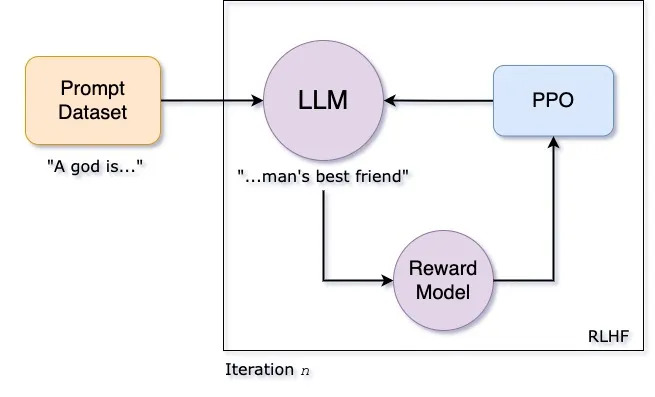
\includegraphics[width=0.485\textwidth]{img/ppo.jpg}
    \caption{PPO Algorithm. https://medium.com/@oleglatypov/a-comprehensive-guide-to-proximal-policy-optimization-ppo-in-ai-82edab5db200}
    \label{fig:ppo}
\end{figure}

\subsubsection{Architettura del modello}
Il cuore del nostro sistema è una rete neurale profonda addestrata attraverso l'algoritmo PPO. La rete neurale accetta input relativi allo stato attuale del veicolo, quali posizione, velocità, angolo di sterzata e dati sensoriali provenienti da telecamere e sensori a ultrasuoni. Il modello produce un'azione di controllo, rappresentata da una distribuzione di probabilità su possibili comandi, consentendo una gestione dinamica e continua del veicolo.

\subsubsection{Addestramento del modello}
Abbiamo utilizzato una vasta raccolta di dati provenienti da simulazioni di guida su diversi circuiti. Ogni episodio di addestramento ha coinvolto il modello che interagisce con l'ambiente simulato, ricevendo ricompense basate su metriche di prestazione come tempi di percorrenza, traiettorie seguite e reazioni a condizioni impreviste come curve strette o variazioni di superficie stradale. L'addestramento è stato eseguito per numerosi cicli, garantendo la convergenza del modello verso strategie ottimali di guida.

\subsubsection{Integrazione dei waypoints}

Un aspetto distintivo della nostra metodologia è l'integrazione dei waypoints dei circuiti nelle mappe di addestramento.
%
Abbiamo identificato e annotato accuratamente i waypoints su ciascun circuito utilizzato, indicando punti chiave sulla traiettoria ottimale.
%
Durante l'addestramento, il modello è stato incentivato a seguire i waypoints, fornendo una guida più precisa e adattandosi alle specificità di ciascun circuito.

\subsubsection{Raccolta e prepoccessing dei dati}
La raccolta dei dati è stata effettuata attraverso simulazioni realistiche, catturando scenari di guida diversificati. I dati sono stati preprocessati per normalizzare le informazioni di input e garantire una distribuzione uniforme delle condizioni di guida, evitando bias durante l'addestramento.

\subsubsection{Parametri e configurazioni}
Abbiamo attentamente selezionato i parametri dell'algoritmo PPO, tra cui il tasso di apprendimento, il coefficiente di entropia e la dimensione dei minibatch, attraverso sperimentazioni iterative per massimizzare le prestazioni del modello su circuiti specifici.

\medskip

Questa metodologia integrata ha consentito l'addestramento di un modello di guida autonoma altamente adattivo, capace di gestire in modo dinamico i circuiti di gara e di ottimizzare le prestazioni in risposta a variazioni ambientali e specificità della pista. Nella sezione successiva, presenteremo i risultati dei nostri esperimenti, evidenziando le capacità e le limitazioni del nostro approccio.

%
%
%
\subsection{Model Usage}

During this phase, the reinforcement learning model trained in the first part of the project becomes the operational core of the car, taking decision on what to do.
%
The application environment is extent to a more complex scenario, based on ROS.

The project is based on F1tenth Gym Ros project \footnote{\url{https://github.com/f1tenth/f1tenth\_gym\_ros}}, a containerized ROS communication bridge for the environment that allow the use of ROS2 API \cite{Ros2}.

The starting point of building a ros node is defining a class that will declare the communication needs, both sending and receiving messages.

\begin{python}
class PPOModelEvaluator(Node):
  def __init__(self):
    super().__init__('car_node')

    #Topics for Pubs & Subs
    lidarscan_topic = '/scan'
    drive_topic = '/drive'

    # Model loading
    self.model = PPO.load(path)

    # ROS2 Sub & Pub
    self.lidar_sub =
      self.create_sub(callback)
    self.drive_pub =
      self.create_pub(...)
\end{python}

After that we can let the control flow spin to handle the specified callback.
%
This node is designed to continuously receive data from the lidar scanner over the vehicle and use the model to predict the optimal actions to be taken based on these inputs.
%
The input data of the model is a vector of $ 1\times1080 $ linear distances between the actual position of the car and first obstacle the light will find over the ray path.
%
It span over an angle of 360 degrees around the car.
%
When new data are ready to be processed, the model start the prediction and the output is the action that the car will take.
%
In this case we can control the steering angle and the speed of the car.

\begin{equation*}
\begin{bmatrix}
    d_1\\
    d_2\\
    \dots\\
    d_{1080}
\end{bmatrix}
\xRightarrow[\text{Prediction}]{\text{Model}}
\begin{pmatrix}
    \texttt{angle}\\
    \texttt{velocity}
\end{pmatrix}
\end{equation*}

\begin{python}
def callback(self, data):
  distances = normalize(data)

  action, _ = self.model.predict(d)
  action = denormalize(action)

  msg = ...
  msg.angle = action[0]
  msg.speed = action[1]
  self.drive_pub.publish(msg)
\end{python}

%
%
%
\section{Esperimenti}

\begin{itemize}
    \item Descrizione delle condizioni sperimentali, tra cui la configurazione dell'addestramento, la scelta dei parametri, ecc.

    \item Presentazione dei risultati ottenuti durante i vostri esperimenti.

    \item Analisi dei risultati, comprese le prestazioni del modello su diversi circuiti.

\end{itemize}

\section{Discussione}

\begin{itemize}
    \item Interpretazione dei risultati e confronto con la letteratura esistente.

    \item Discussione sulle sfide incontrate e le eventuali limitazioni del vostro approccio.

    \item Possibili sviluppi futuri e miglioramenti proposti.

\end{itemize}

\section{Conclusioni}

\begin{itemize}
    \item Riassunto dei risultati principali.

    \item Sottolineare l'importanza del vostro contributo e le potenziali implicazioni nella guida autonoma.

\end{itemize}

\bibliographystyle{IEEEtran}
\bibliography{bibliography}

\end{document}
